\section{Initial test on May 7th}
On May 7th the group met up to perform the first real test of the system, aiming to try out the full experience of the game, using the VR goggles to view the game and using the Pozyx system to generate positional data based on the movement of the players.
This test was conducted with the goal of exposing issues with the state of the system, as well as simply test whether or not it would be playable, meaning the player characters would move in a regular fashion without jerking around the screen.
A testing area was constructed in order to conduct the test.
One part of this area can be seen on \autoref{fig:test1-roomsetup}, while \autoref{fig:test1-singlepozyx} shows how we mounted the anchors onto a wall for the setup.
\begin{figure}[]
    \centering
    \includegraphics[scale=0.06]{/sprint4/first-test/IMG_20200507_135004.jpg}
    \caption{A view of the room used for the test. Two anchors can be seen on the sides.}
    \label{fig:test1-roomsetup}
\end{figure}
\begin{figure}[]
    \centering
    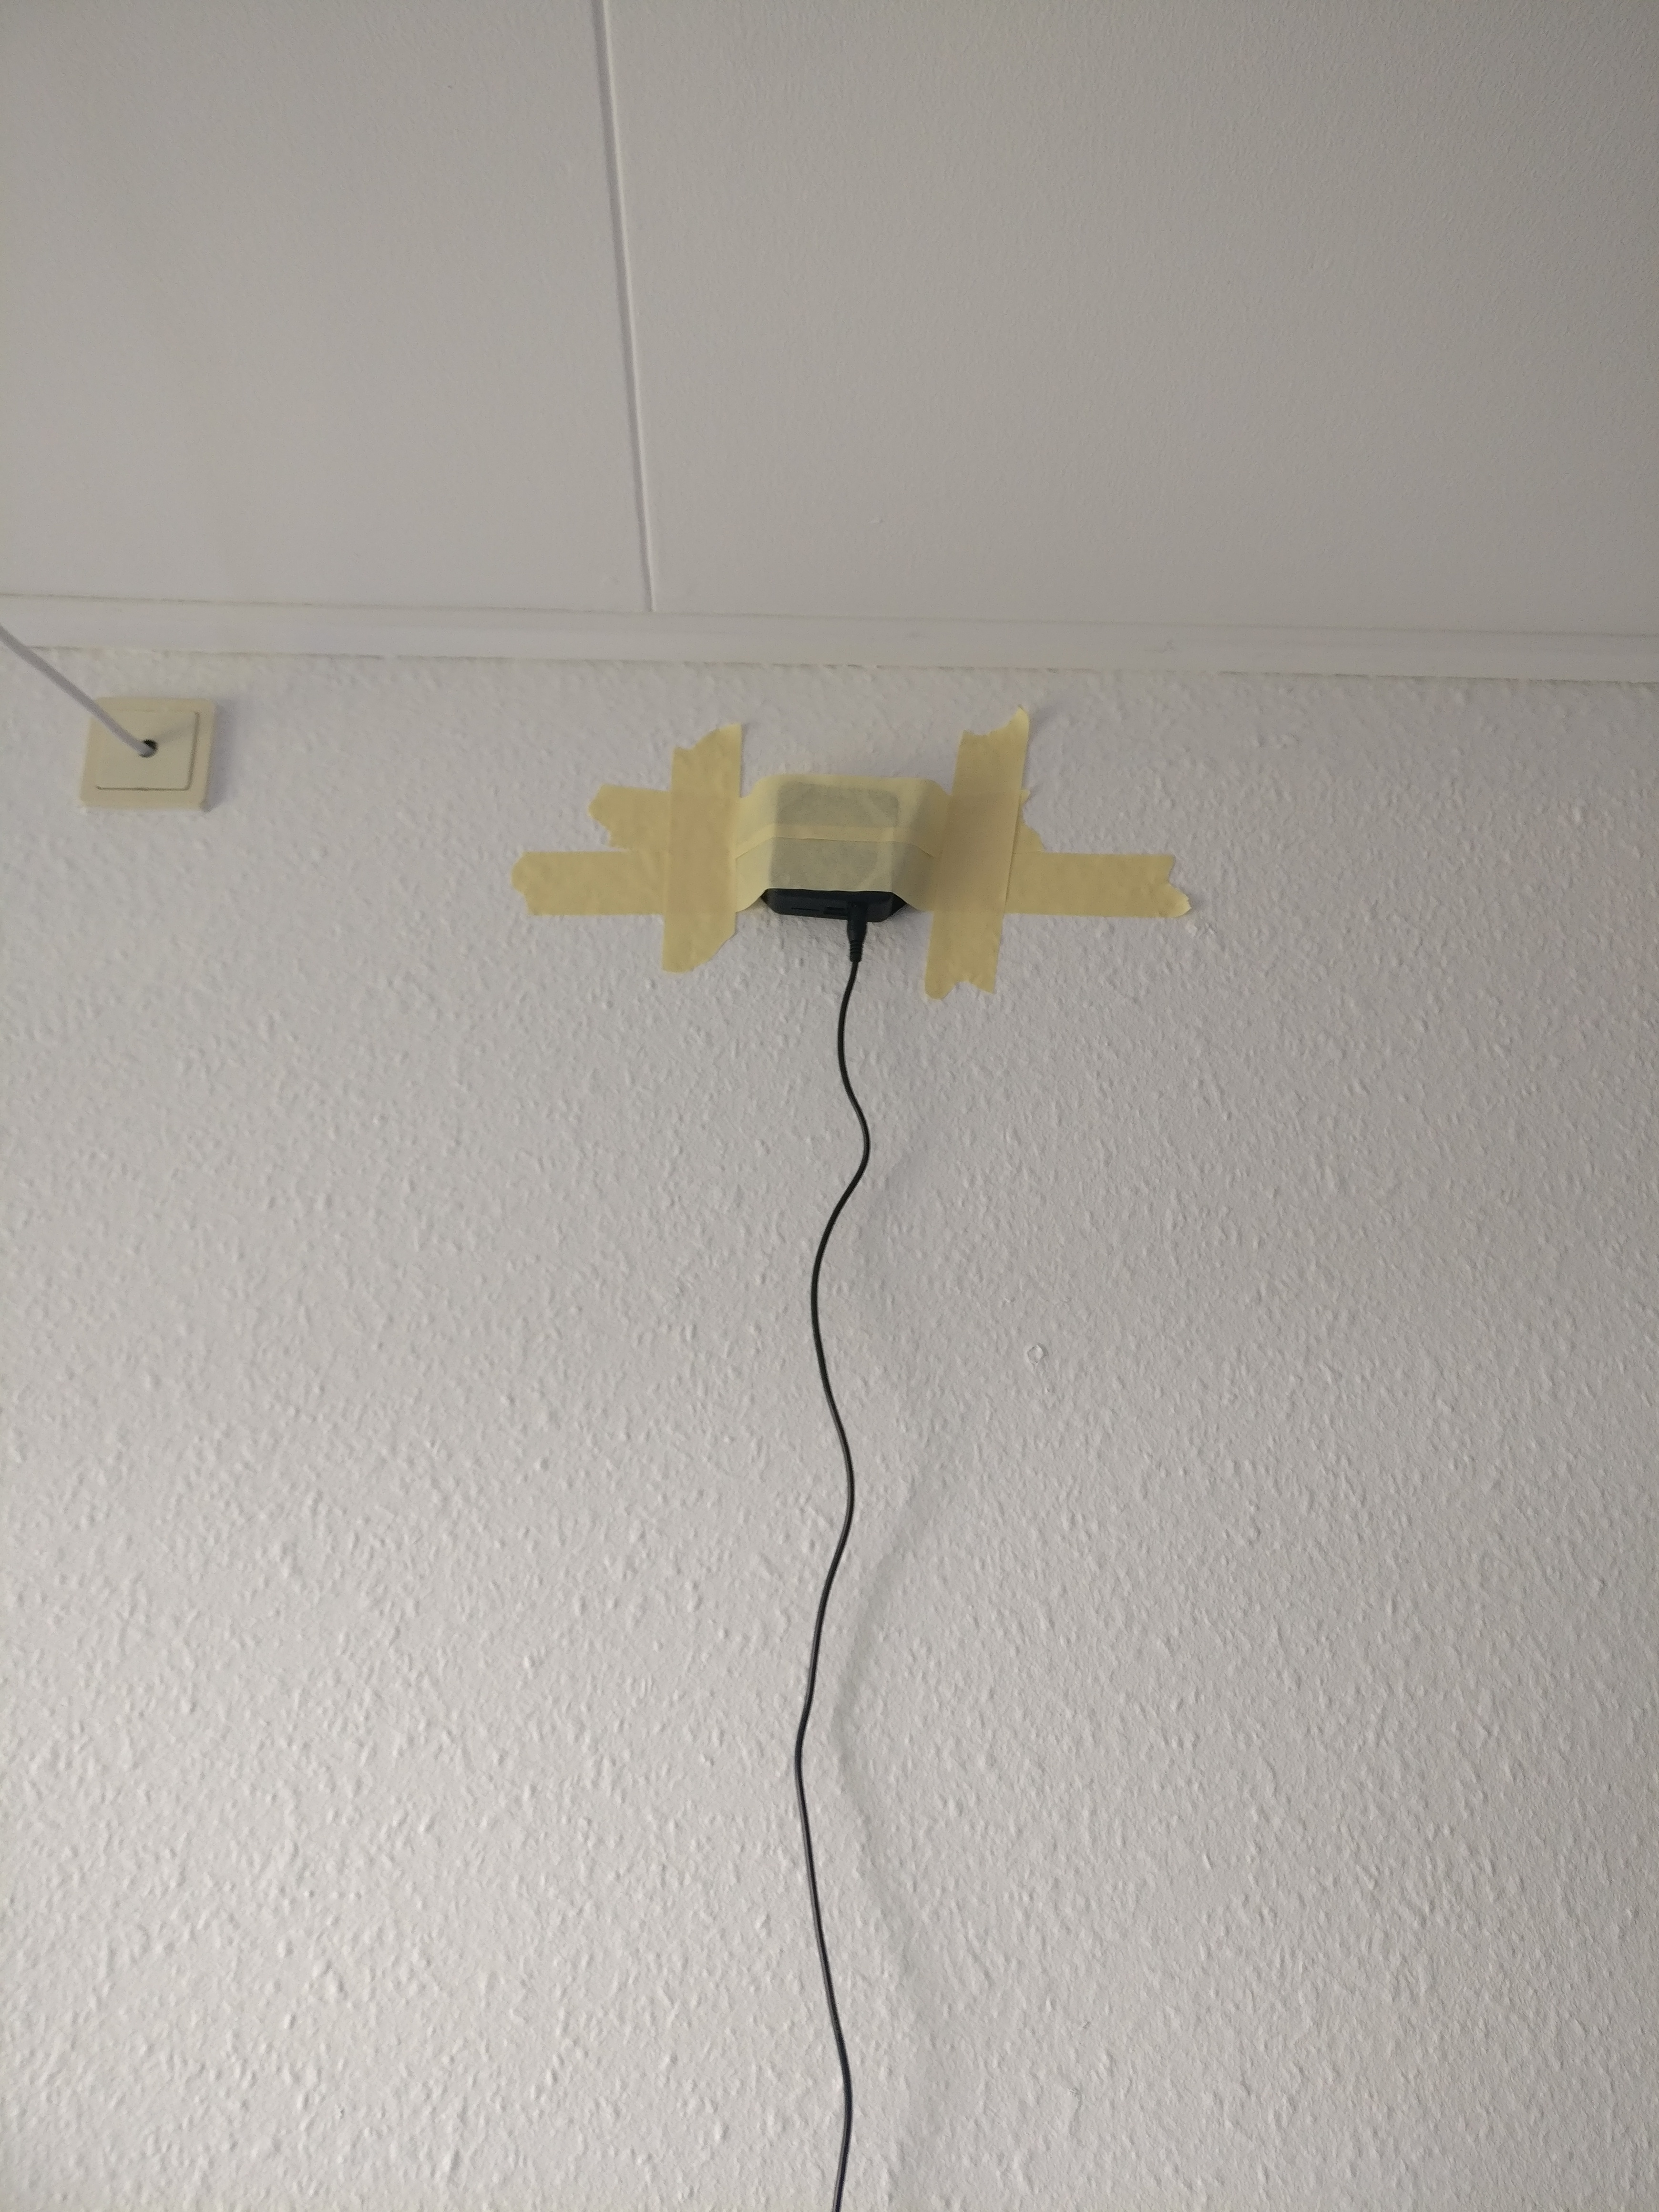
\includegraphics[scale=0.05]{/sprint4/first-test/IMG_20200507_134955.jpg}
    \caption{A single Pozyx anchor has been attached to a wall.}
    \label{fig:test1-singlepozyx}
\end{figure}
\noindent
The final area was documented, with the details shown on \autoref{fig:test1-paperofsetup}.
\begin{figure}[]
    \centering
    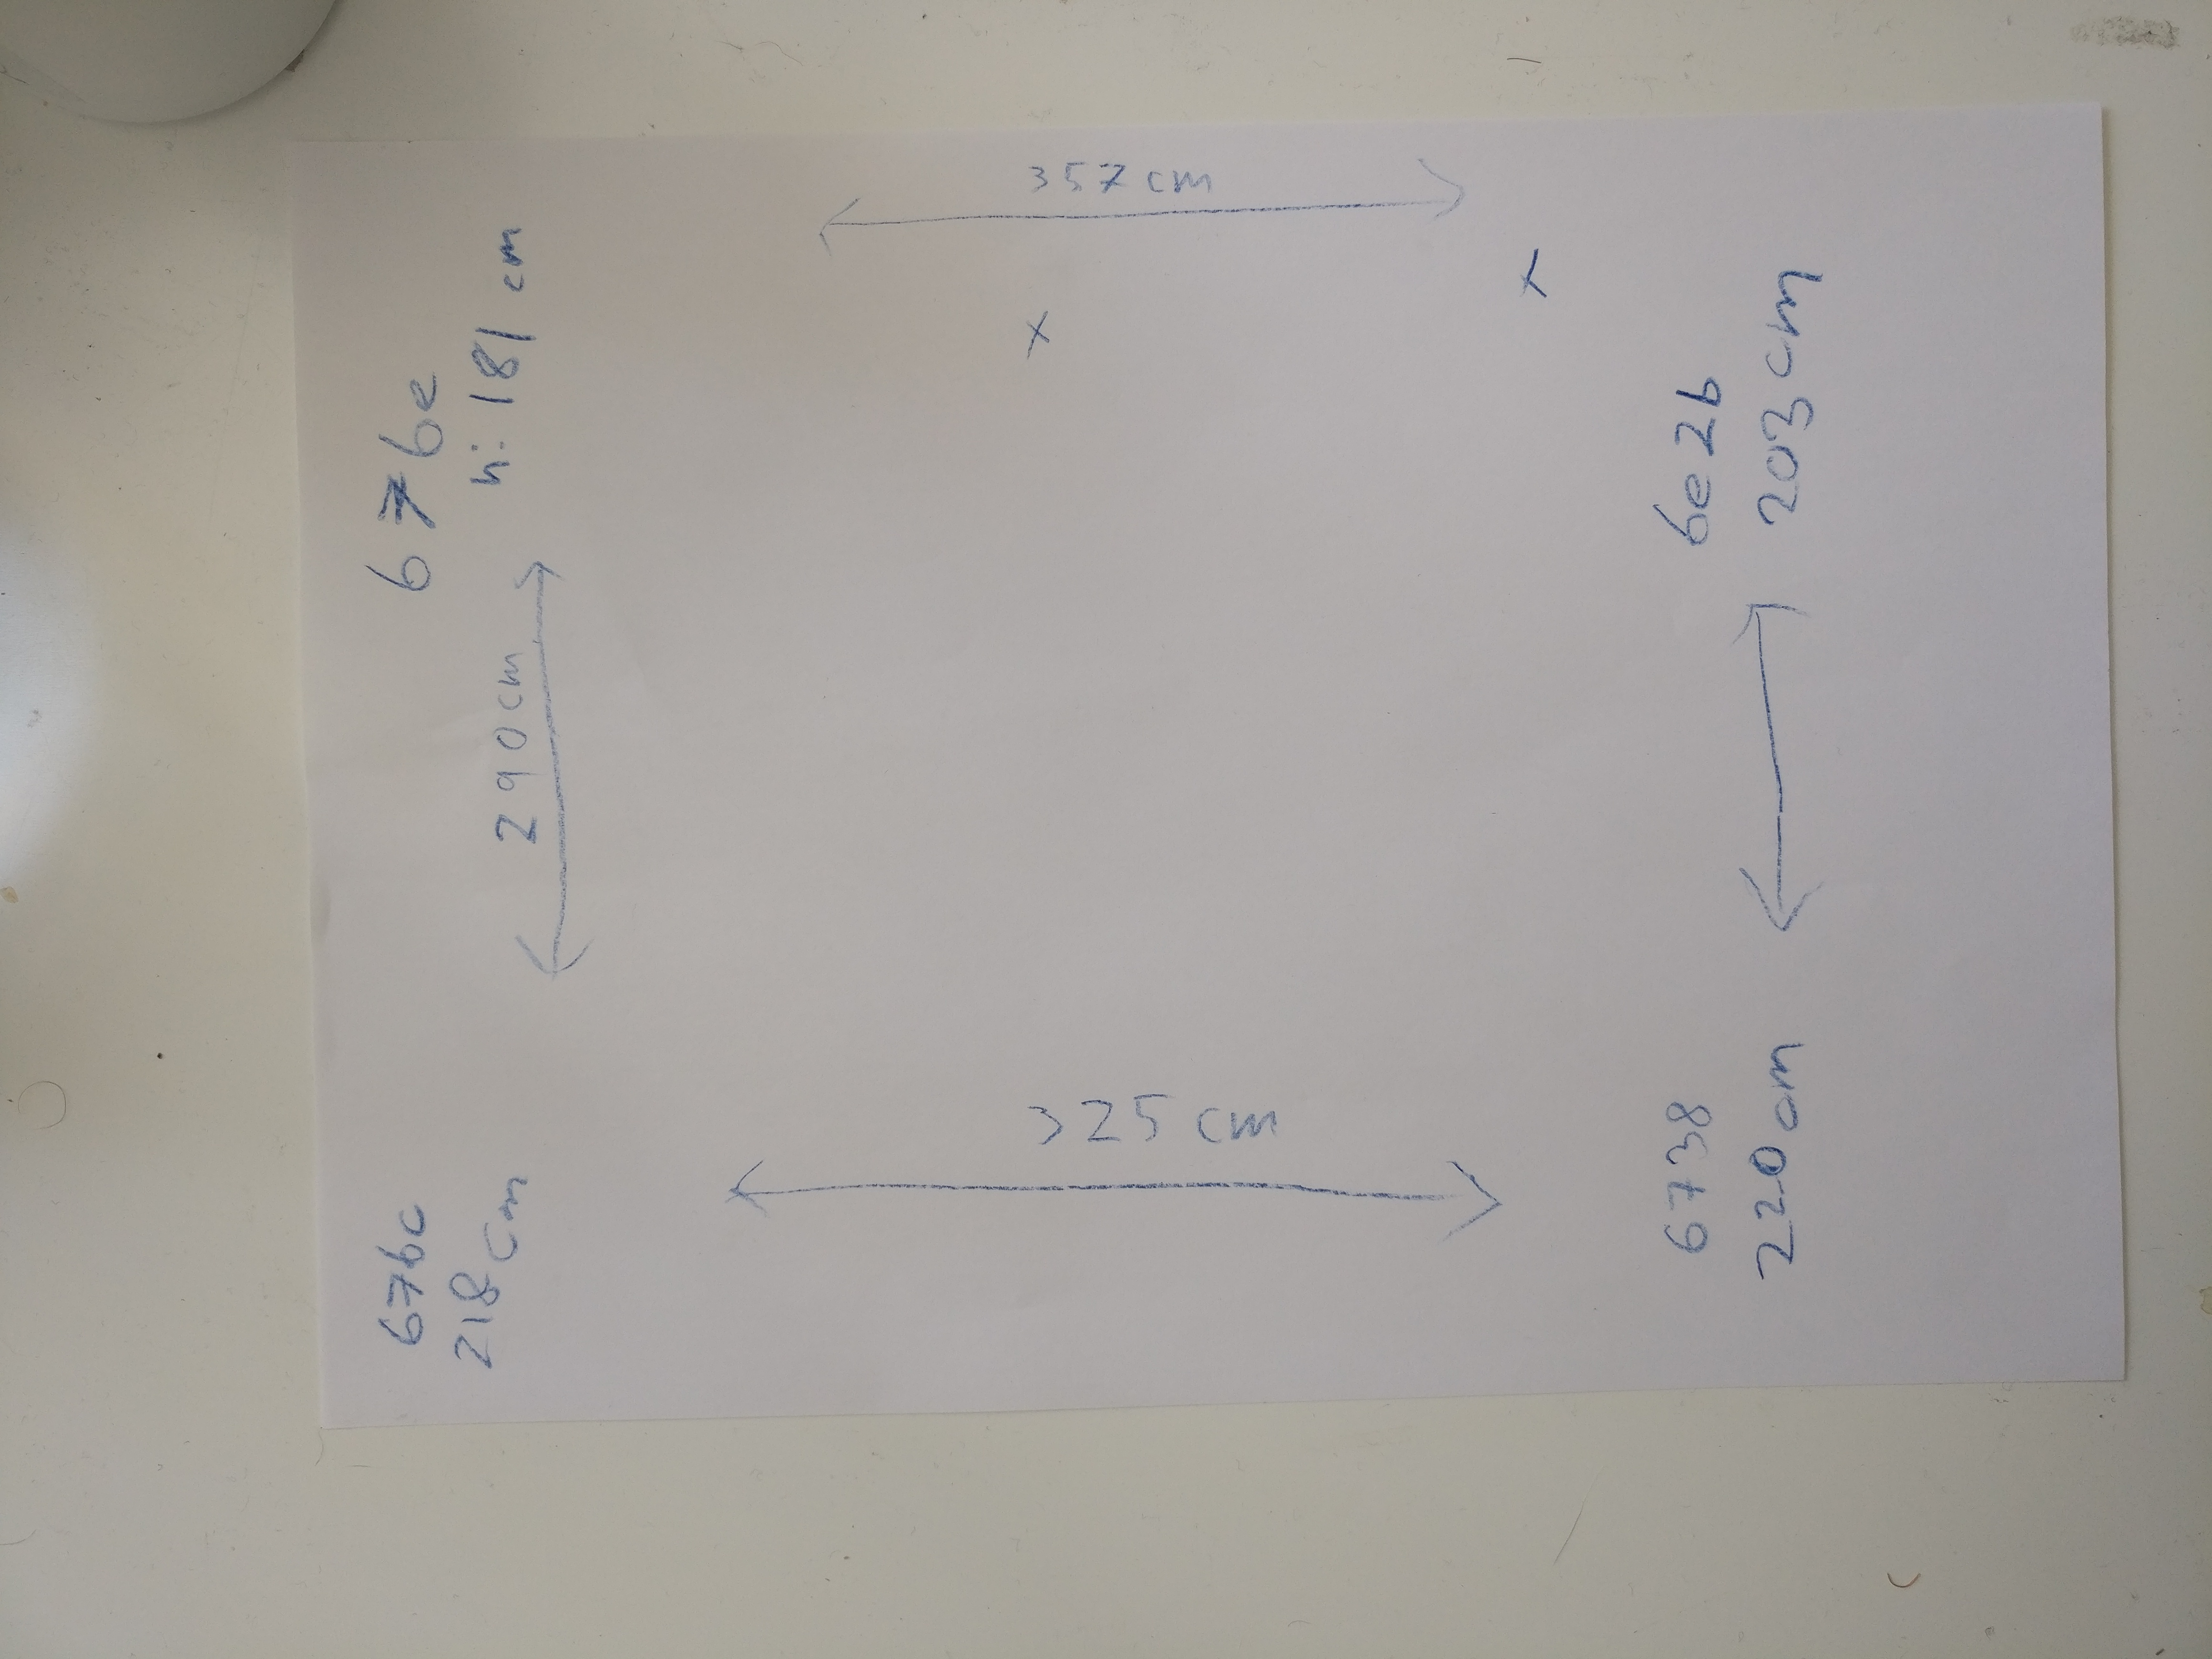
\includegraphics[width=\linewidth]{/sprint4/first-test/IMG_20200507_135024.jpg}
    \caption{A paper defining the setup, noting height of anchors, anchor tags and distance between anchors.}
    \label{fig:test1-paperofsetup}
\end{figure}
\noindent
The documentation of distance is necessary for the host to know how to input the anchor positions in the setup of the game, and the anchors are placed high on the walls, to increase the chance of receiving a good signal \cite{pozyx-AnchorHeights}.
In order to view the game, the test made use of four sets of VR goggles, shown on \autoref{fig:test1-goggles}
\begin{figure}[]
    \centering
    \includegraphics[scale=0.04]{/sprint4/first-test/IMG_20200507_135402.jpg}
    \caption{The VR goggles used to hold and view the phone.}
    \label{fig:test1-goggles}
\end{figure}
\noindent

\subsubsection{The results of the test}
The overall goal of this test was to play the game in a two versus two fashion.
This test, however, did not quite accomplish that goal.
Leading up to the test, members of the group had communicated regarding a smaller scale test, only involving a single person, that would test that the Pozyx system generated data and passed it along to Unity.
This seemed to work, so the actual test was carried out with more people.
There had been a miscommunication however, the smaller scale test was carried out on test data, making use of predefined data that had been used during development.
When the day of the test came, it turned out this would be the first test with real data based on an actual game setup.
This led to the encountering of several bugs.
\\\\
The first, and most time consuming, was caused by some firmware issues with the Pozyx anchors, delaying the test until they had been updated.
Then issues were encountered when trying to send the host configuration data to the players.
This was caused by some unintended type conversions in the Python code.
Another issue related to the input from the host.
There was no specific information regarding the unit which should be used when inputting information, such as centimeters, millimeters or meters, and this caused some confusion.
Finally, once four players were able to connect and receive configuration data from the host, the game launched for the players, but they were immobile, not moving on the field based on the Pozyx data.
Another issue encountered during testing was related to the blue goal zone.
This goal zone specifically could flicker when the player moved his head, which the red zone did not.
As such, while the test did not achieve the original goal, it still exposed certain issues to fix for the upcoming sprint. 